

%% AAPT Physics Bowl Exams Questions
%%----------------------------------------


%% This section has XX problems


%% PhysicsBowl 2015
%%----------------------------------------
\element{aapt}{ %% Bowl-D4
\begin{question}{bowl-2015-q29}
    An electron moves at constant non-zero velocity directly between two long straight wires.
    The conventional current in each wire has the same magnitude,
        but the currents are in opposite directions as shown in the figure.
    \begin{center}
    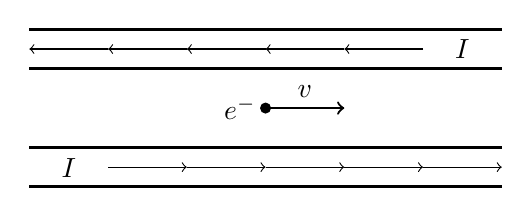
\begin{tikzpicture}
        %% NOTE: rotated 90 degrees
        %% electron
        \fill (0,0) circle (2pt) node[anchor=east] {$e^{-}$};
        \draw[thick,->] (0,0) -- (1,0) node[pos=0.5,anchor=south] {$v$};
        %% upper wire
        \draw[very thick] (-3,1) -- (3,1);
        \draw[very thick] (-3,0.5) -- (3,0.5);
        \node[anchor=south] at (+2.5,0.5) {$I$};
        \foreach \x in {-2,-1,...,2} {
            \draw[->] (\x,+0.75) -- ++(180:1);
        }
        %% lower wire
        \draw[very thick] (-3,-1) -- (3,-1);
        \draw[very thick] (-3,-0.5) -- (3,-0.5);
        \node[anchor=south] at (-2.5,-1.0) {$I$};
        \foreach \x in {-2,-1,...,2} {
            \draw[->] (\x,-0.75) -- ++(0:1);
        }
    \end{tikzpicture}
    \end{center}
    Ignoring gravity, which choice best reflects the direction of the magnetic field
        and the direction of the electric field that exist at the location of the electron?
    Any electric field in the region originates from an unseen external source.
    \begin{center}
    \begin{tabu}{cX[c]X[2c]}
        \toprule
        \makebox[1.5em][c]{\textnumero}
            & Electric Field & Magnetic Field \\
        \bottomrule
    \end{tabu}
    \end{center}
    \begin{choices}
        \wrongchoice{\begin{tabu}{X[c]X[2c]} No Field & No Field \\ \end{tabu}}
        \wrongchoice{\begin{tabu}{X[c]X[2c]} To the left & Into the plane of the page \\ \end{tabu}}
        \wrongchoice{\begin{tabu}{X[c]X[2c]} To the right & Into the plane of the page \\ \end{tabu}}
        \wrongchoice{\begin{tabu}{X[c]X[2c]} To the left & Out of the plane of the page \\ \end{tabu}}
      \correctchoice{\begin{tabu}{X[c]X[2c]} To the right & Out of the plane of the page \\ \end{tabu}}
    \end{choices}
\end{question}
}


%% PhysicsBowl 2014
%%----------------------------------------
\element{aapt}{ %% Bowl-D4
\begin{question}{bowl-2014-q24}
    For the bar magnet shown in the figure,
        which choice best describes the direction of the magnetic field at the point $P$ located directly above the center of the magnet?
    \begin{center}
    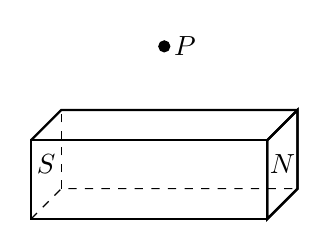
\begin{tikzpicture}
        %% Cube
        \draw[thick] (0,0,0) -- (3,0,0) -- (3,1,0) -- (0,1,0) -- cycle;
        \draw[thick] (3,0,0) -- (3,0,-1) -- (3,1,-1) -- (3,1,0) -- cycle;
        \draw[thick] (3,0,0) -- (3,0,-1) -- (3,1,-1) -- (3,1,0) -- cycle;
        \draw[thick] (0,1,0) -- (0,1,-1) -- (3,1,-1);
        \draw[dashed] (0,0,0) -- (0,0,-1) -- (3,0,-1);
        \draw[dashed] (0,0,-1) -- (0,1,-1);
        %% Labels
        \draw[fill] (1.5,2.0,-0.5) circle (2pt) node[anchor=west] {$P$};
        \node[anchor=center] at (3.0,0.5,-0.5) {$N$};
        \node[anchor=center] at (0.0,0.5,-0.5) {$S$};
    \end{tikzpicture}
    \end{center}
    \begin{choices}
        \wrongchoice{Up the plane of the page}
        \wrongchoice{To the right}
        \wrongchoice{Down the plane of the page}
      \correctchoice{To the left}
        \wrongchoice{Out of the plane of the page}
    \end{choices}
\end{question}
}

\element{aapt}{ %% Bowl-D4
\begin{question}{bowl-2014-q29}
    An electron with charge $-e$ and mass $m$ travels at a speed $v$
        in a plane perpendicular to the magnetic field of magnitude $B$.
    The electron follows a circular path of radius $R$.
    In a time $t$, the electron travels halfway around the circle.
    What is the amount of work done by the magnetic force on the
        electron in this time?
    \begin{multicols}{2}
    \begin{choices}
      \correctchoice{zero}
        \wrongchoice{$-\pi evBR$}
        \wrongchoice{$\pi evBR$}
        \wrongchoice{$-2\pi evBR$}
        \wrongchoice{$\dfrac{\pi mv}{eB}$}
    \end{choices}
    \end{multicols}
\end{question}
}


%% PhysicsBowl 2013
%%----------------------------------------
\element{aapt}{ %% Bowl-D4
\begin{question}{bowl-2013-q30}
    Electrons flow to the left in a wire as shown.
    \begin{center}
    \begin{tikzpicture}
        %% Wire
        \draw (-3.5,+0.5) -- (+3.5,+0.5);
        \draw (-3.5,-0.5) -- (+3.5,-0.5);
        %% Current
        \foreach \x in {30,20,10,0,-10,-20}
            \draw[xshift=-0.25cm,thick,->] (\x mm,0) -- ++ (180:0.75cm);
        \draw[fill] (3,0) circle (1.5pt)
            node[anchor=west] {$e^-$};
        %% Electron
        \draw[fill] (0,1) circle (1pt)
            node[anchor=west] {$p^+$};
            %node[anchor=west] {proton};
        \draw[thick,->] (0,1) -- ++ (90:1cm)
            node[pos=0.5,anchor=west] {$v$};
    \end{tikzpicture}
    \end{center}
    For the proton moving toward the top of the page at the instant shown,
        what is the direction of the magnetic force on the proton?
    \begin{choices}
        \wrongchoice{To the left}
      \correctchoice{To the right}
        \wrongchoice{Into the plane of the page}
        \wrongchoice{Out of the plane of the page}
        \wrongchoice{There is no force}
    \end{choices}
\end{question}
}


%% PhysicsBowl 2012
%%----------------------------------------
\element{aapt}{ %% Bowl-D4
\begin{question}{bowl-2012-q28}
    A long straight wire has a conventional current
        directed into the plane of the page as shown in the figure.
    \begin{center}
    \begin{tikzpicture}
        %% Point P with vectors
        \draw[fill] (0,0) circle (1.5pt) node[anchor=west] {$P$};
        \draw[thick,->] (0,0) -- ++ (90:2) node[anchor=south] {$A$};
        \draw[thick,->] (0,0) arc (0:30:4) node[anchor=south east] {$B$};
        \draw[thick,->] (0,0) -- ++ (180:2) node[anchor=east] {$C$};
        \draw[thick,->] (0,0) arc (0:-30:4) node[anchor=north east] {$D$};
        \draw[thick,->] (0,0) -- ++ (270:2) node[anchor=north] {$E$};
        %% Wire X
        \draw[thick] (-3,0) circle (1ex);
        \foreach \x in {45,135,225,315}
            \draw[thick] (-3,0) -- ++ (\x:0.5ex);
        \path (-3,0) ++(120:1ex) node[pin={120:wire}]  {};
    \end{tikzpicture}
    \end{center}
    Which one of the arrows shown best indicates the
        direction of the magnetic field associated
        with this wire at the location labeled $P$?
    \begin{multicols}{5}
    \begin{choices}[o]
        \wrongchoice{$A$}
        \wrongchoice{$B$}
        \wrongchoice{$C$}
        \wrongchoice{$D$}
      \correctchoice{$E$}
    \end{choices}
    \end{multicols}
\end{question}
}

\element{aapt}{ %% Bowl-D4
\begin{question}{bowl-2012-q36}
    A positive charge moves with constant velocity through a region of space containing both an electric field and a magnetic field.
    The electric field is directed out of the plane of the page.
    Ignoring any gravitational field,
        which one of the following choices represents possible directions of both the particle's velocity and the total magnetic field in the region of space?
    \begin{center}
    \begin{tabu}{cX[c]X[c]}
        \toprule
        \makebox[1.5em][c]{\textnumero}
            & Velocity of particle
            & Magnetic Field \\
        \bottomrule
    \end{tabu}
    \end{center}
    \begin{choices}
        \wrongchoice{\begin{tabu}{X[c]X[c]} Toward the bottom of the page & Into the plane of the page \\ \end{tabu}}
        \wrongchoice{\begin{tabu}{X[c]X[c]} Into the plane of the page & Out of the plane of the page \\ \end{tabu}}
        \wrongchoice{\begin{tabu}{X[c]X[c]} To the left & Toward the bottom of the page \\ \end{tabu}}
      \correctchoice{\begin{tabu}{X[c]X[c]} Toward the top of the page & To the right \\ \end{tabu}}
        \wrongchoice{\begin{tabu}{X[c]X[c]} Out of the plane of the page & Toward the top of the page \\ \end{tabu}}
    \end{choices}
\end{question}
}


%% PhysicsBowl 2011
%%----------------------------------------
\element{aapt}{ %% Bowl-D4
\begin{question}{bowl-2011-q29}
    An electron moves with speed \SI{1.00e3}{\meter\per\second} as it enters a region of space that has only a uniform magnetic field.
    The electron is accelerated because of this field with a constant magnitude of \SI{3.00e5}{\meter\per\second\squared} for the entire time of \SI{1.00e-3}{\second} that it is in the field.
    With what speed would the electron exit the field?
    Ignore gravity?
    \begin{choices}
        \wrongchoice{\SI{1.80e3}{\meter\per\second}}
        \wrongchoice{\SI{1.41e3}{\meter\per\second}}
      \correctchoice{\SI{1.00e3}{\meter\per\second}}
        \wrongchoice{\SI{2.00e2}{\meter\per\second}}
        \wrongchoice{It depends on the initial angle of the electron's velocity with respect to the magnetic field.}
    \end{choices}
\end{question}
}

\element{aapt}{ %% Bowl-D4
\begin{question}{bowl-2011-q34}
    A wire lies in the plane of the page with conventional current $I$ as shown below.
    \begin{center}
    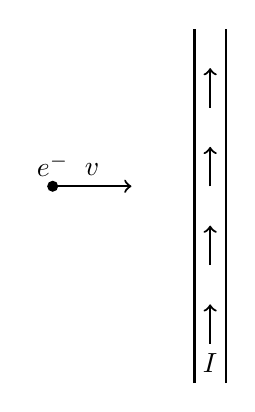
\begin{tikzpicture}
        %% wire
        \foreach \x in {-0.2,0.2} \draw[thick] (\x,-2.5) -- (\x,2.0);
        \foreach \x in {-2,-1,0,1} \draw[thick,->] (0,\x) -- ++(90:0.5);
        \node[anchor=north] at (0,-2) {$I$};
        %% electron
        \fill (-2,0) circle (2pt) node[anchor=south] {$e^{-}$};
        \draw[thick,->] (-2,0) -- ++(0:1) node[pos=0.5,anchor=south] {$v$};
    \end{tikzpicture}
    \end{center}
    At the instant shown,
        what is the direction of the magnetic force on the electron that is moving directly to the right toward the wire?
    \begin{choices}
        \wrongchoice{Toward the bottom of the page}
      \correctchoice{Toward the top of the page}
        \wrongchoice{Into the plane of the page}
        \wrongchoice{Out of the place of the page}
        \wrongchoice{There is no force}
    \end{choices}
\end{question}
}


%% PhysicsBowl 2010
%%----------------------------------------
\element{aapt}{ %% Bowl-D4
\begin{question}{bowl-2010-q43}
    Two ions travel perpendicular to the same uniform magnetic field.
    The ions carry the same charge and have the same path radius in the magnetic field.
    Which of the following quantities \emph{must} be the same for the two ions?
    \begin{choices}
        \wrongchoice{Mass}
        \wrongchoice{Speed}
        \wrongchoice{Charge-to-mass ratio}
        \wrongchoice{Kinetic energy}
      \correctchoice{Magnitude of linear momentum}
    \end{choices}
\end{question}
}


%% PhysicsBowl 2009
%%----------------------------------------
\element{aapt}{ %% Bowl-D4
\begin{question}{bowl-2009-q27}
    A proton moves straight up the plane of this page into a region
        that has a magnetic field directed to the right.
    If the particle is undeflected as it passes through this region,
        in what direction must there be a component of electric field?
    Ignore gravity.
    \begin{multicols}{2}
    \begin{choices}
        \wrongchoice{To the left}
        \wrongchoice{Into the page}
      \correctchoice{Out of the page}
        \wrongchoice{Down the page}
        \wrongchoice{To the right}
    \end{choices}
    \end{multicols}
\end{question}
}


%% PhysicsBowl 2006
%%----------------------------------------
\element{aapt}{ %% Bowl-D4
\begin{question}{bowl-2006-q37}
    For the four identical current-carrying wires shown (with conventional current coming out of the plane of the page),
        the wire on the right is labeled $P$.
    \begin{center}
    \begin{tikzpicture}
        %% currents
        \foreach \x in {0,90,180,270} {
            \draw (\x:1.5) circle (1ex);
            \fill (\x:1.5) circle (1.6pt);
            \node[anchor=center,shift={(\x:-1em)}] at (\x:1.5) {\SI{4}{\ampere}};
        }
        %% point P
        \node[anchor=west,xshift=1ex] at (0:1.5) {$P$};
    \end{tikzpicture}
    \end{center}
    What is the direction of the magnetic force on the wire labeled $P$ from the other wires?
    \begin{choices}
      \correctchoice{To the left}
        \wrongchoice{To the right}
        \wrongchoice{Up the plane of the page}
        \wrongchoice{Down the plane of the page}
        \wrongchoice{There is no force.}
    \end{choices}
\end{question}
}


%% PhysicsBowl 1999
%%----------------------------------------
\element{aapt}{ %% Bowl-D4
\begin{question}{bowl-1999-q29}
    Two light wires are hung vertically.
    With electrical current in both wires directed upward:
    \begin{choices}
      \correctchoice{the wires will experience a force of attraction}
        \wrongchoice{the wires will experience a force of repulsion}
        \wrongchoice{the force on the right hand wire will cancel the force on the left hand wire}
        \wrongchoice{both wires will experience a torque until they are at right angles to one another}
        \wrongchoice{none of the provided are true}
    \end{choices}
\end{question}
}


%% PhysicsBowl 1998
%%----------------------------------------
\element{aapt}{ %% Bowl-D4
\begin{question}{bowl-1998-q10}
    A charged particle with constant velocity enters a uniform magnetic field whose direction is parallel to the particle's velocity.
    The particle will:
    \begin{choices}
        \wrongchoice{speed up}
        \wrongchoice{slow down}
      \correctchoice{experience no change in velocity}
        \wrongchoice{follow a parabolic arc.}
        \wrongchoice{follow a circular arc.}
    \end{choices}
\end{question}
}


%% PhysicsBowl 1997
%%----------------------------------------
\element{aapt}{ %% Bowl-D4
\begin{question}{bowl-1997-q02}
    An electric current flows through a horizontal wire
        from left to right as shown in the accompanying diagram.
    \begin{center}
    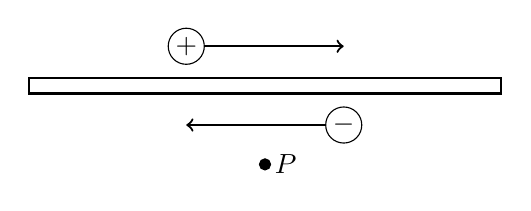
\begin{tikzpicture}
        %% NOTE: how they represent current is interesting
        \draw[thick] (-3,-0.1) rectangle (3,0.1);
        \node[anchor=center,circle,draw,inner sep=1pt] (A) at (-1,0.50) {$+$};
        \draw[thick,->] (A) -- ++ (0:2cm);
        \node[anchor=center,circle,draw,inner sep=1pt] (B) at (1,-0.50) {$-$};
        \draw[thick,->] (B) -- ++ (180:2cm);
        \draw[fill] (0,-1.00) circle (2pt) node[anchor=west] {$P$};
    \end{tikzpicture}
    \end{center}
     Which option best represents the direction of the
        magnetic field at $P$?
    \begin{choices}
      \correctchoice{into the page}
        \wrongchoice{out of the page}
        \wrongchoice{to the right of the page}
        \wrongchoice{toward the top of the page}
        \wrongchoice{toward the bottom of the page}
    \end{choices}
\end{question}
}

\element{aapt}{ %% Bowl-D4
\begin{question}{bowl-1997-q17}
    Two bar magnets are to be cut in half along the dotted lines shown below.
    \begin{center}
    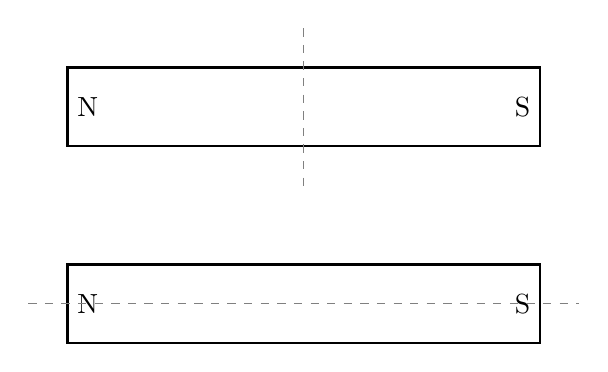
\begin{tikzpicture}
        %% Vertical
        \begin{scope}[yshift=1.25cm]
            \draw[thick] (-3,0.5) rectangle (3,-0.5);
            \node[anchor=east] at (3,0) {S};
            \node[anchor=west] at (-3,0) {N};
            \draw[dashed,white!50!black] (0,1) -- (0,-1);
        \end{scope}
        %% horizontal
        \begin{scope}[yshift=-1.25cm]
            \draw[thick] (-3,0.5) rectangle (3,-0.5);
            \node[anchor=east] at (3,0) {S};
            \node[anchor=west] at (-3,0) {N};
            \draw[dashed,white!50!black] (-3.5,0) -- (3.5,0);
        \end{scope}
    \end{tikzpicture}
    \end{center}
    None of the pieces are rotated.
    After the cut:
    \begin{choices}
        \wrongchoice{None of the halves will attract any other.}
        \wrongchoice{The two halves of each magnet will attract each other.}
        \wrongchoice{The two halves of each magnet will repel each other.}
        \wrongchoice{The two halves of the top magnet will repel, the two halves of the bottom magnet will attract.}
      \correctchoice{The two halves of the top magnet will attract, the two halves of the bottom magnet will repel.}
    \end{choices}
\end{question}
}

\element{aapt}{ %% Bowl-D4
\begin{question}{bowl-1997-q28}
    An ion with charge $q$, mass $m$,
        and speed $v$ enters a magnetic field $B$ and is deflected into a path with a radius of curvature $R$.
    If a second ion has speed $2v$, while $m$, $q$, and $B$ are unchanged,
        what will be the radius of the second ion's path?
    \begin{multicols}{3}
    \begin{choices}
        \wrongchoice{$4R$}
      \correctchoice{$2R$}
        \wrongchoice{$R$}
        \wrongchoice{$\dfrac{R}{2}$}
        \wrongchoice{$\dfrac{R}{4}$}
    \end{choices}
    \end{multicols}
\end{question}
}

\element{aapt}{ %% Bowl-D4
\begin{question}{bowl-1997-q32}
    A wire moves through a magnetic field directed into the page.
    The wire experiences an induced charge separation as shown.
    \begin{center}
    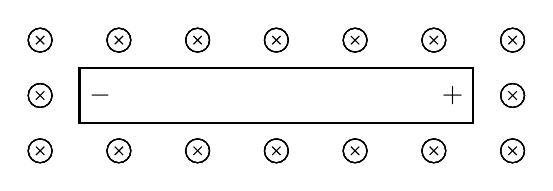
\begin{tikzpicture}
        %% metal bar
        \draw[thick] (-2.5,-1em) rectangle (2.5,1em);
        \node[anchor=west] at (-2.5,0) {$-$};
        \node[anchor=east] at (+2.5,0) {$+$};
        %% B field into page
        \foreach \x in {-30,-20,...,30}
            \foreach \y in {-2em,2em}
                \foreach \i in {45,135,225,315} {
                    \draw (\x mm,\y) -- ++(\i:0.5ex);
                    \draw (\x mm,\y) circle (1ex);
                }
        \foreach \x in {-30,30}
            \foreach \i in {45,135,225,315} {
                \draw (\x mm,0) circle (1ex);
                \draw (\x mm,0) -- ++(\i:0.5ex);
            }
    \end{tikzpicture}
    \end{center}
    Which way is the wire moving?
    \begin{choices}
        \wrongchoice{to the right}
        \wrongchoice{to the left}
        \wrongchoice{out of the page}
        \wrongchoice{toward the top of the page}
      \correctchoice{toward the bottom of the page}
    \end{choices}
\end{question}
}


%% PhysicsBowl 1996
%%----------------------------------------
\element{aapt}{ %% Bowl-D4
\begin{question}{bowl-1996-q07}
    An amber rod is given a net negative charge and held at rest.
    Which of the following statements is true?
    \begin{choices}
        \wrongchoice{The amber rod is surrounded only by a magnetic field that circles the rod.}
        \wrongchoice{The amber rod is surrounded only by an electric field that is directed out from the rod.}
      \correctchoice{The amber rod is surrounded only by an electric field that is directed into the rod.}
        \wrongchoice{The amber rod is surrounded by both a magnetic field that circles the rod and an electric field that is directed out from the rod.}
        \wrongchoice{The amber rod is surrounded by both a magnetic field that circles the rod and an electric field that is directed into the rod.}
    \end{choices}
\end{question}
}

\element{aapt}{ %% Bowl-D4
\begin{question}{bowl-1996-q40}
    A proton of mass $M$ and kinetic energy $E_k$ passes undeflected through a region with electric and magnetic fields perpendicular to each other.
    The electric field has magnitude $E$.
    The magnitude of the magnetic field $B$ is:
    \begin{multicols}{3}
    \begin{choices}
        \wrongchoice{$\sqrt{\dfrac{ME^2}{E_k}}$}
        \wrongchoice{$\sqrt{\dfrac{ME}{2E_k}}$}
        \wrongchoice{$\sqrt{\dfrac{2ME}{E_k}}$}
      \correctchoice{$\sqrt{\dfrac{ME^2}{2E_k}}$}
        \wrongchoice{$\sqrt{\dfrac{ME^2}{E_k^2}}$}
    \end{choices}
    \end{multicols}
\end{question}
}


%% PhysicsBowl 1995
%%----------------------------------------
\element{aapt}{ %% Bowl-D4
\begin{question}{bowl-1995-q16}
    A charged particle with constant speed enters a uniform magnetic field whose direction is perpendicular to the particle's velocity.
    The particle will:
    \begin{choices}
        \wrongchoice{Speed up.}
        \wrongchoice{Slow down.}
        \wrongchoice{Experience no change in velocity.}
        \wrongchoice{Follow a parabolic arc.}
      \correctchoice{Follow a circular arc.}
    \end{choices}
\end{question}
}

\element{aapt}{ %% Bowl-D4
\begin{question}{bowl-1995-q30}
    A \SI{0.20}{\meter} long copper rod has constant velocity \SI{0.30}{\meter\per\second} traveling through a uniform magnetic field of \SI{0.060}{\tesla}.
    The rod, velocity, and magnetic field are all mutually perpendicular.
    What is the potential difference induced across the rod’s length?
    \begin{multicols}{2}
    \begin{choices}
      \correctchoice{\SI{0.0036}{\volt}}
        \wrongchoice{\SI{0.040}{\volt}}
        \wrongchoice{\SI{0.090}{\volt}}
        \wrongchoice{\SI{1.0}{\volt}}
        \wrongchoice{\SI{25}{\volt}}
    \end{choices}
    \end{multicols}
\end{question}
}


%% PhysicsBowl 1994
%%----------------------------------------
\element{aapt}{ %% Bowl-D4
\begin{question}{bowl-1994-q29}
    Four infinitely long wires are arranged as shown in the accompanying figure's end-on view.
    %% NOTE: bowl-2006-q37
    \begin{center}
    \begin{tikzpicture}
        %% currents
        \foreach \x in {45,135,225,315} {
            \node[anchor=center,shift={(\x:-1em)}] at (\x:2) {$I$};
            \draw (\x:2) circle (1ex);
            \pgfmathifthenelse{\x == 45}{}{"\noexpand\fill (\x:2) circle (1.5pt);"}\pgfmathresult
        }
        \foreach \x in {45,135,225,315} \draw (45:2) -- ++(\x:0.66ex);
        %% point P
        \node[anchor=center] at (0,0) {$P$};
    \end{tikzpicture}
    \end{center}
    All four wires are perpendicular to the plane of the page and have the same magnitude of current $I$.
    The conventional current in the wire in the upper right-hand corner is directed into the plane of the page.
    The other conventional currents are out of the plane of the page.
    Point $P$ is a distance a from all four wires.
    What is the total magnetic field at point $P$?
    \begin{choices}
        \wrongchoice{$\dfrac{\mu_0}{2\pi} I^2$ toward the wire}
        \wrongchoice{$\dfrac{\mu_0 I^2 L}{2\pi R}$ upward, in the same direction as $I$}
      \correctchoice{$\dfrac{\mu_0 I^2 L}{2\pi R}$ downward, in the opposite direction as $I$}
        \wrongchoice{$ev \dfrac{\mu_0 I L}{2\pi R}$ upward, in the same direction as $I$}
        \wrongchoice{$ev \dfrac{\mu_0 I L}{2\pi R}$ downward, in the opposite direction as $I$}
    \end{choices}
\end{question}
}


\endinput


